\subsubsection{SIR Model}
We begin with a simple model of a disease in a population of size $N$.
We divide the population into three classes: susceptible $S$, infected $I$, and recovered $R$.
Let
\begin{equation*}
	\begin{aligned}
		\beta&=\text{infection rate}\quad\mu=\text{death rate}\quad\upsilon=\text{recovery rate}\\
		\gamma&=\text{rate by which recovered individuals have lost their immunity and became susceptible to the disease.}
	\end{aligned}
\end{equation*}
Then we have the following diagram:
\begin{figure}[H]
	\centering
	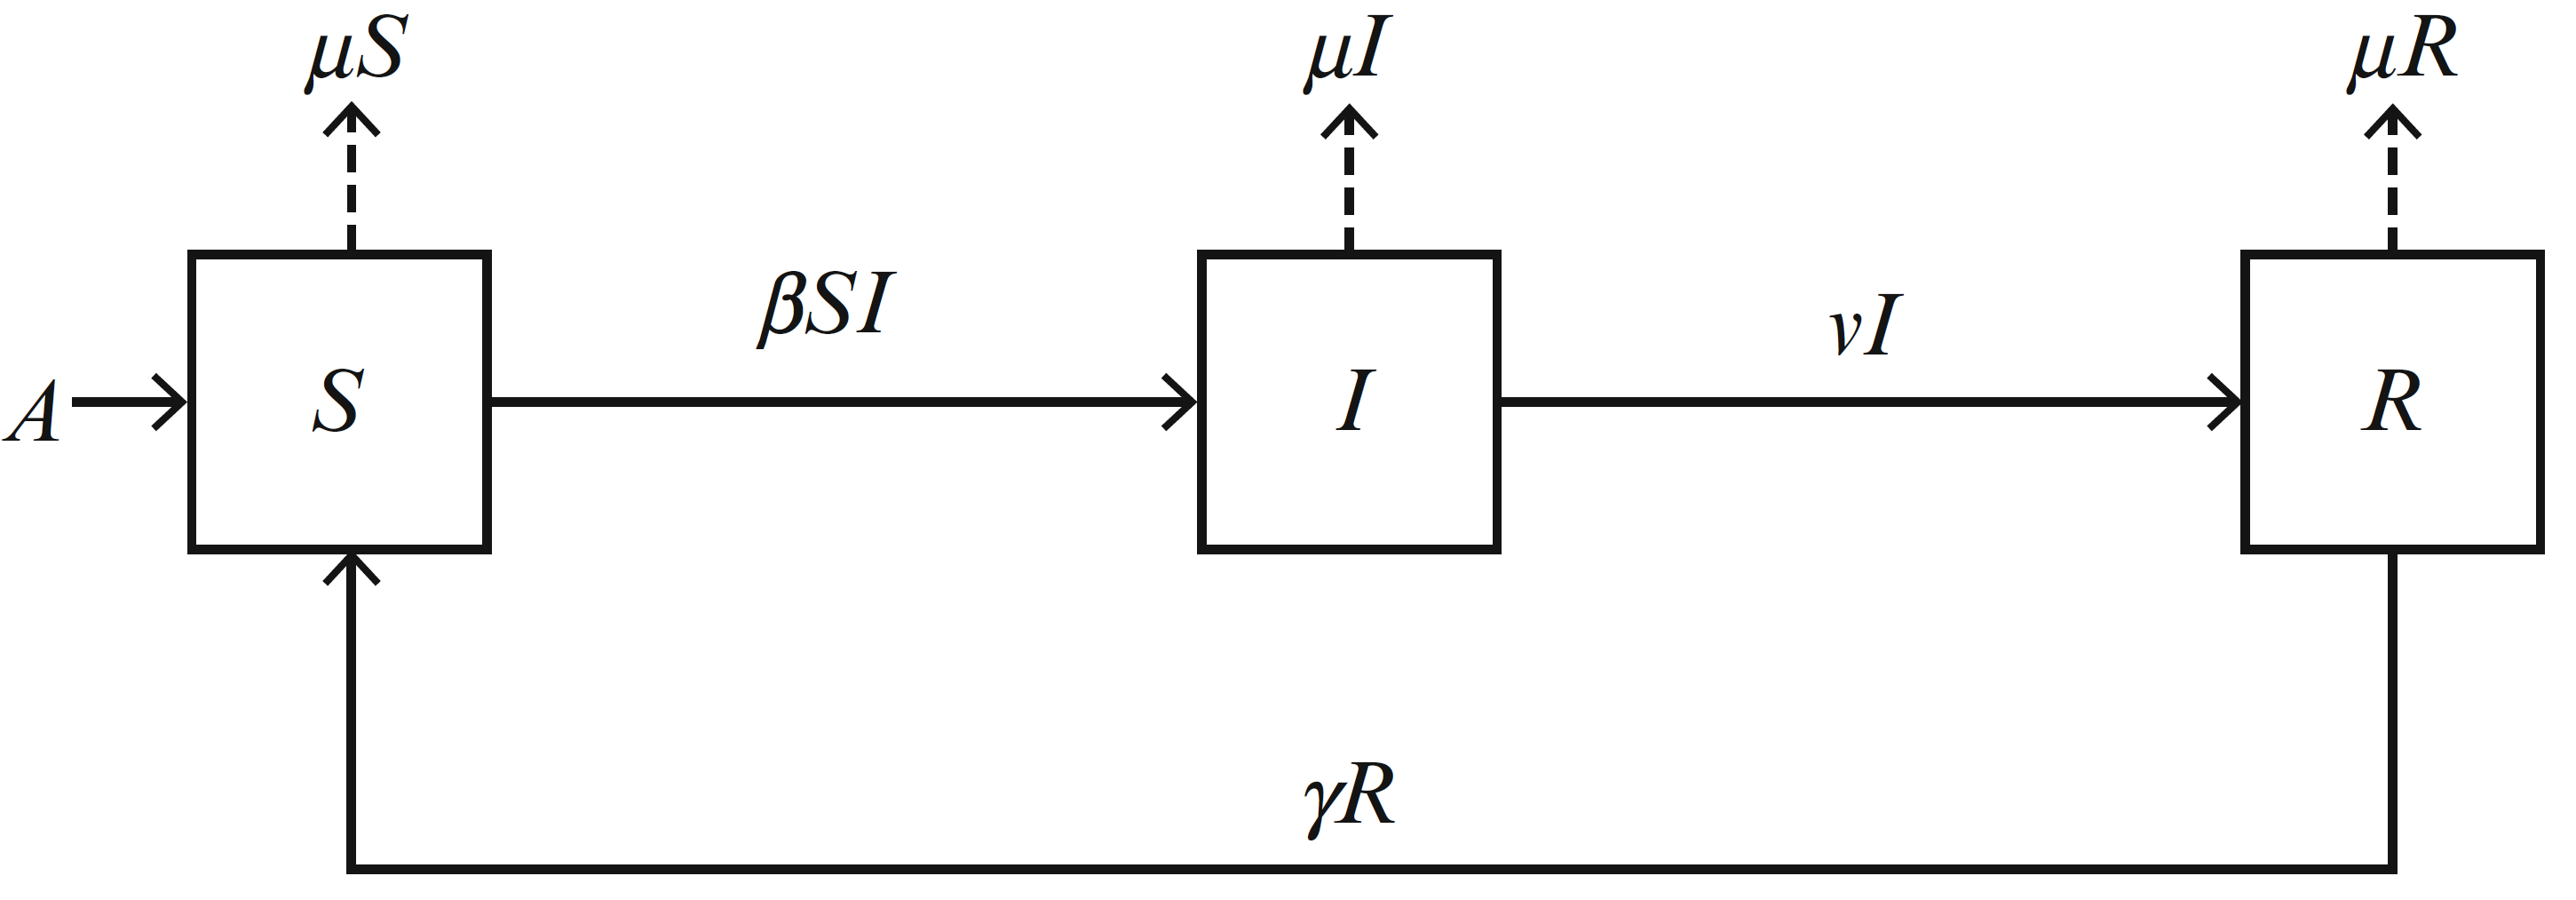
\includegraphics[width=0.5\linewidth]{sirbd.png}
	%\caption{}
	\label{fig:sirbd}
\end{figure}
where $A$ is the growth of susceptible.
If all newborns are healthy, then not only $S$ and $R$,but also $I$ contributes to the growth term $A$.
We view each of the populations $S$, $I$, $R$, $N$ as representing a number of individuals (or a number density, that is, the number of individuals per unit area).
The dimension of $\gamma,\mu,\upsilon$ is $1/$time, the dimension of $\beta$ is 1$/$(individual$\cdot$time), and the dimension of $A$ is individual$/$time.
\begin{equation}{\label{eq:sirm}}
	\begin{aligned}
		\frac{dS}{dt}&=A-\beta SI+\gamma R-\mu S\\
		\frac{dI}{dt}&=\beta SI-\upsilon I-\mu I\\
		\frac{dR}{dt}&=\upsilon I-\gamma R-\mu R
	\end{aligned}
\end{equation}
To examine more carefully the meaning of $A$, we introduce a differential equation
for $N(t)$, which is obtained by adding all the equations in (\ref{eq:sirm})
\begin{equation}
	\frac{dN}{dt}=A-\mu N\quad\rightarrow\quad N(t)=N_0e^{-\mu t}+\frac{A}{\mu}(1-e^{-\mu t})
\end{equation}
Hence $N(t)\rightarrow A/\mu$ as $t\rightarrow\infty$. Thus $A/\mu$ is equal to the asymptotic density of the population (as $t\rightarrow\infty$).\\
The SIR model has an equilibrium point which is disease free, namely
\begin{equation}
	(S_0,I_0,R_0)=\left(\frac{A}{\mu},0,0\right)
\end{equation}
we call it the \textbf{disease free equilibrium} (DFE). The Jacobian matrix at the DFE is
\begin{equation}
	J(S_0,I_0,R_0)=
	\begin{pmatrix}
		-\mu&-\beta\dfrac{A}{\mu}&\gamma\\
		0&\beta\dfrac{A}{\mu}-(\upsilon+\mu)&0\\
		0&\upsilon&-\mu-\gamma\\
	\end{pmatrix}\quad\rightarrow\quad\text{The eigenvalues are}\quad
	\begin{aligned}
		\lambda_1&=-\mu\\
		\lambda_2&=-\mu-\gamma\\
		\lambda_3&=\beta\frac{A}{\mu}-(\upsilon+\mu)
	\end{aligned}
\end{equation}
Hence, the DFE is stable if
\begin{equation}{\label{eq:sirdfes}}
	\lambda_{1,2,3}<0\quad\rightarrow\quad\beta\frac{A}{\mu}<\upsilon+\mu
\end{equation}
We conclude that in order to stop the spread of infection we need to either decrease the rate of infection ($\beta$) by decreasing contact between healthy and infected individuals, or by increasing the rate of recovery ($\upsilon$) by drugs.
When (\ref{eq:sirdfes}) holds, any new small infection will die out with time.\\
On the other hand if,
\begin{equation}{\label{eq:sirdfeus}}
	\beta\frac{A}{\mu}>\upsilon+\mu
\end{equation}
the DFE is unstable; there are arbitrarily small infections that will not disappear in the population.\\
Furthermore, there is an equilibrium point $(\tilde{S},\tilde{I},\tilde{R})$ with $\tilde{I}>0$, namely
\begin{equation}
	\beta\tilde{S}=\upsilon+\mu\quad\tilde{R}=\frac{\upsilon}{\gamma+\mu}\tilde{I}\quad\frac{\beta}{\mu}\tilde{I}=\frac{\left(\beta\dfrac{A}{\mu}-(\upsilon+\mu)\right)}{\upsilon+\mu-\dfrac{\gamma\upsilon}{\gamma+\mu}}
\end{equation}
\begin{theorem}
	If (\ref{eq:sirdfeus}) holds then the equilibrium point $(\tilde{S},\tilde{I},\tilde{R})$ is stable.
\end{theorem}
\begin{proof}
	The Jacobian matrix at $(\tilde{S},\tilde{I},\tilde{R})$
	\begin{equation}
		J(\tilde{S},\tilde{I},\tilde{R})=
		\begin{pmatrix}
			-\beta\tilde{I}-\mu&-\beta\tilde{S}&\gamma\\
			\beta\tilde{I}&\beta\tilde{S}-(\upsilon+\mu)&0\\
			0&\upsilon&-\mu-\gamma\\
		\end{pmatrix}\quad\text{with}\quad \beta\tilde{S}=\upsilon+\mu
	\end{equation}
	Hence the characteristic polynomial is
	\begin{equation}
		\det(J(\tilde{S},\tilde{I},\tilde{R})-\lambda I)=0\quad\rightarrow\quad\lambda^3+\alpha_1\lambda^2+\alpha_2\lambda+\alpha_3=0\quad\text{where}\quad
		\begin{aligned}
			\alpha_1&=(\beta\tilde{I}+\mu)+(\gamma+\mu)\\
			\alpha_2&=(\beta\tilde{I}+\mu)(\gamma+\mu)+\beta\tilde{I}(\upsilon+\mu)\\
			\alpha_3&=\beta\tilde{I}[(\upsilon+\mu)(\gamma+\mu)-\upsilon\gamma]
		\end{aligned}
	\end{equation}
	Clearly all the $\alpha_i$ are positive, and
	\begin{equation}
		\alpha_1\alpha_2=\beta\tilde{I}(\upsilon+\mu)(\gamma+\mu)+\text{positive terms}>\beta\tilde{I}[(\upsilon+\mu)(\gamma+\mu)-\upsilon\gamma]=\alpha_3.
	\end{equation}
	Hence, by the Routh-Hurwitz criterion\footnote{More about Routh-Hurwitz criterion \href{https://en.wikipedia.org/wiki/Routh-Hurwitz_stability_criterion}{here}}, the equilibrium point $(\tilde{S},\tilde{I},\tilde{R})$ is stable.
\end{proof}
A stable equilibrium point with $I>0$ is called \textbf{endemic}; it represents a disease that will never disappear.\\
In a healthy population we introduce one infection and compute the expected infection among the susceptibles caused by this single infection.
We call it the \textbf{expected secondary infection}, or \textbf{basic reproduction number}, and denote it by $R_0$.
Then intuitively it is clear that DFE is \emph{stable} if $R_0<1$ (the secondary infection is smaller than the initial infection) whereas if $R_0>1$ then the DFE will be \emph{unstable}.
Clearly, $R_0=\beta\dfrac{A}{\mu(\upsilon+\mu)}$.
\subsubsection{SEIR Model}
When a susceptible is exposed to an infected individual, he/she may or may not become immediately sick.
With this in mind, we may extend the SIR model by introducing a new class $E$ of exposed individuals.
The new model, called the \textbf{SEIR} model, consists of the following equations:
\begin{equation}{\label{eq:seirm}}
	\begin{aligned}
		\frac{dS}{dt}&=A-\beta SI+\gamma R-\mu S\\
		\frac{dE}{dt}&=\beta SI-\kappa E-\mu  E\\
		\frac{dI}{dt}&=\kappa E-\upsilon I-\mu I\\
		\frac{dR}{dt}&=\upsilon I-\gamma R-\mu R
	\end{aligned}
\end{equation}
Here $\kappa$ is the rate by which the exposed become infected, and $\beta$ is the rate of infection of susceptibles by infected individuals.
The DFE for the SEIR model is $\left(\dfrac{A}{\mu},0,0,0\right)$.
Here $R_0=\beta\dfrac{A\kappa}{\mu(\upsilon+\mu)(\kappa+\mu)}$.\\
So far we considered infectious diseases that do not cause death.
In infectious diseases which cause \textbf{death}, e.g., Ebola, we need to change the equation for $I$ by including a death rate $\rho$ caused by the disease.
Then the equation for $I$ in the system (\ref{eq:sirm}) becomes
\begin{equation}
	\frac{dI}{dt}=\beta SI-\gamma I-\mu I-\rho I
\end{equation}
Here, $R_0=\beta\dfrac{A}{\mu(\upsilon+\mu+\rho)}$.